\documentclass{beamer}
\usetheme{Madrid}

\usepackage{amsmath, amssymb, amsthm}
\usepackage{graphicx}
\usepackage{listings}
\usepackage{gensymb}
\usepackage[utf8]{inputenc}
\usepackage{hyperref}
\usepackage{tikz}
\lstset{
	language=Python,
	basicstyle=\ttfamily\small,
	keywordstyle=\color{blue},
	stringstyle=\color{orange},
	numbers=left,
	numberstyle=\tiny\color{gray},
	breaklines=true,
	showstringspaces=false
}
\usetikzlibrary{decorations.pathmorphing}

\title{Question-12.9.ex.19}
\author{EE24BTECH11030 - J.KEDARANANDA}
\date{}
\begin{document}
	
	\frame{\titlepage}
	
	\begin{frame}
		\frametitle{Question}
		Find the maximum area of an isosceles triangle inscribed in the ellipse $\frac{x^2}{a^2}+\frac{y^2}{b^2}=1$with its vertex at one end of the major axis.\\
	\end{frame}
	\begin{frame}{Theoretical Solution}
		\textbf{Theoretical solution:}
		
		Consider the isosceles triangle ABC: \\
		$A(a, 0)$, $B(a \cos\theta, b \sin\theta)$, and $C(a \cos\theta, -b \sin\theta)$ \\
		
		\begin{align}
			\text{Area of } \triangle ABC &= \frac{1}{2} \times BC \times \text{height of } \triangle ABC \\
			\text{Height of } \triangle ABC &= a(1 - \cos\theta) \\
			BC &= 2b \sin\theta \\
			\Delta &= \frac{1}{2} \times 2b \sin\theta \times a(1 - \cos\theta) \\
			&= ab \sin\theta (1 - \cos\theta)
		\end{align}
	\end{frame}
	\begin{frame}{Theoretical Solution: Maximum Area}
		For the maximum area of the triangle:
		\begin{align}
			\frac{d\Delta}{d\theta} &= ab \cos\theta (1 - \cos\theta) + ab \sin^2\theta = 0 \\
			\cos\theta (1 - \cos\theta) + \sin^2\theta &= 0 \\
			\cos\theta &= \cos{2\theta}
		\end{align}
		
		\begin{align}
			\cos\theta &= -\frac{1}{2}
		\end{align}
		
		For the maximum value:
		\begin{align}
			\cos\theta &= -\frac{1}{2}, \quad \sin\theta = \frac{\sqrt{3}}{2} \\
			\text{Maximum area} &= ab \times \frac{\sqrt{3}}{2} \left( 1 + \frac{1}{2} \right) \\
			&= \frac{3\sqrt{3}}{4} ab
		\end{align}
	\end{frame}
	\begin{frame}{Computational Solution}
		\textbf{Computational solution:}
		\newline
		By the gradient descent algorithm, the difference equation is given by,
		\begin{align}
			f(x) &= ab \sin{x} (1 - \cos{x}) \\
		\end{align}
		to find the value of $x_n$ for the maximum area:
		\begin{align}
			x_{n + 1} &= x_n + \mu f^{\prime}\left(x_{n}\right) \\
			x_{n + 1} &= x_n + \mu \left(ab \cos{x_{n}} (1 - \cos{x_{n}}) + ab \sin^2{x_{n}}\right)
		\end{align}
		\[
		x_{n+1} = x_n + \mu ab \cos x_n (1 - \cos x_n) + \mu ab \sin^2 x_n
		\]
		Taking the Z-transform on both sides:
		\[
		zX(z) - zx_0 = X(z) + \mu ab \cos(X(z))(1 - \cos(X(z))) + \mu ab \sin^2(X(z)).
		\]
		\begin{align}
			(Z-1)X(Z)-Zx_{0}={\mu}ab\left(\frac{1-Z^{-1}\cos{1}}{1-2Z^{-1}\cos{1}+Z^{-2}}-\frac{1-Z^{-1}\cos{2}}{1-Z^{-1}\cos{2}+Z^{-2}}\right)
		\end{align}
	\end{frame}
	\begin{frame}{Convergence of the Sequence}
		If the sequence $x_n$ has to converge:
		\begin{align}
			\lim_{n\to\infty} \abs{x_{n + 1} - x_n} &= 0 \\
			\implies \lim_{n\to\infty} \abs{{\mu}ab(\cos(2x_{n})-\cos(x_{n}))} &= 0 \\
			\implies \mu \lim_{n\to\infty} \abs{{\mu}ab(\cos(2x_{n})-\cos(x_{n}))} &= 0 \text{, } \mu > 0 \\
			\implies \lim_{n\to\infty} \cos(2x_{n})-\cos(x_{n}) &= 0 \\
			\implies \lim_{n\to\infty} x_{n} &= \frac{2\pi}{3}
		\end{align}
	\end{frame}
	\begin{frame}{Computational Solution for Minimum Area}
		To find the value of $x_n$ for the minimum area:
		\begin{align}
			x_{n + 1} &= x_n - \mu f^{\prime}(x_{n}) \\
			x_{n + 1} &= x_n - \mu \left( ab \cos{x_{n}} (1 - \cos{x_{n}}) + ab \sin^2{x_{n}} \right)
		\end{align}
		\[
		x_{n+1} = x_n - \mu ab \cos x_n (1 - \cos x_n) + \mu ab \sin^2 x_n
		\]
		Taking the Z-transform on both sides:
		\[
		zX(z) - zx_0 = X(z) - \mu ab \cos(X(z))(1 - \cos(X(z))) + \mu ab \sin^2(X(z)).
		\]
		\begin{align}
			(Z-1)X(Z) - Zx_{0} = -{\mu}ab\left(\frac{1-Z^{-1}\cos{1}}{1-2Z^{-1}\cos{1}+Z^{-2}} - \frac{1-Z^{-1}\cos{2}}{1-Z^{-1}\cos{2}+Z^{-2}} \right)
		\end{align}
	\end{frame}
	\begin{frame}{Computational Solution for Minimum Area (Convergence Condition)}
		If the sequence $x_n$ has to converge, we have:
		\begin{align}
			\lim_{n \to \infty} \abs{x_{n + 1} - x_n} &= 0 \\
			\implies \lim_{n \to \infty} \abs{-{\mu}ab(\cos(2x_{n}) - \cos(x_{n}))} &= 0 \\
			\implies \mu \lim_{n \to \infty} \abs{-{\mu}ab(\cos(2x_{n}) - \cos(x_{n}))} &= 0 \text{, } \mu > 0 \\
			\implies \lim_{n \to \infty} \cos(2x_{n}) - \cos(x_{n}) &= 0 \\
			\implies \lim_{n \to \infty} x_{n} &= 0
		\end{align}
	\end{frame}
	\begin{frame}
		\frametitle{Diagram}
		\begin{figure}[!ht]
			\centering
			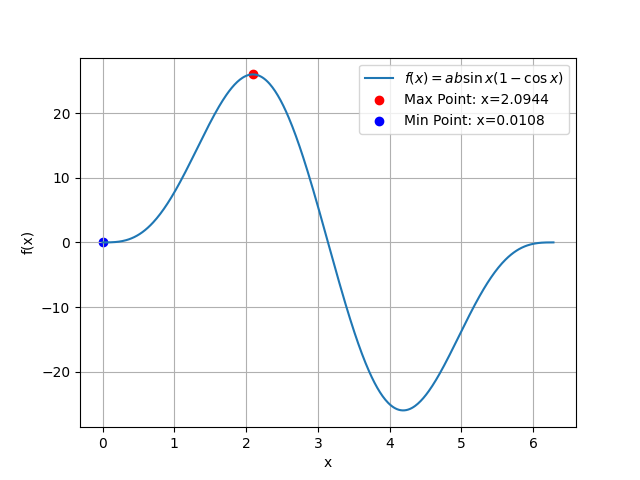
\includegraphics[width=\linewidth]{figs/Fig.png}
		\end{figure}
	\end{frame}
\end{document}

